\documentclass{amsart}
% !TEX root = ../msimplicial.tex

\usepackage{microtype}
\usepackage{amssymb}
\usepackage{mathtools}
\usepackage{tikz-cd}
\usepackage{mathbbol} % changes \mathbb{} and adds more support

% bibliography
\usepackage[
	backend=biber,
	style=alphabetic,
	backref=true,
	url=false,
	doi=false,
	isbn=false,
	eprint=false]{biblatex}

\renewbibmacro{in:}{}  % don't display "in:" before the journal name
\AtEveryBibitem{\clearfield{pages}}  % don't show page numbers

\DeclareFieldFormat{title}{\myhref{\mkbibemph{#1}}}
\DeclareFieldFormat
[article,inbook,incollection,inproceedings,patent,thesis,unpublished]
{title}{\myhref{\mkbibquote{#1\isdot}}}

\newcommand{\doiorurl}{%
	\iffieldundef{url}
	{\iffieldundef{eprint}
		{}
		{http://arxiv.org/abs/\strfield{eprint}}}
	{\strfield{url}}%
}

\newcommand{\myhref}[1]{%
	\ifboolexpr{%
		test {\ifhyperref}
		and
		not test {\iftoggle{bbx:eprint}}
		and
		not test {\iftoggle{bbx:url}}
	}
	{\href{\doiorurl}{#1}}
	{#1}%
}

% references
\usepackage[
	bookmarks=true,
	linktocpage=true,
	bookmarksnumbered=true,
	breaklinks=true,
	pdfstartview=FitH,
	hyperfigures=false,
	plainpages=false,
	naturalnames=true,
	colorlinks=true,
	pagebackref=false,
	pdfpagelabels]{hyperref}

\hypersetup{
	colorlinks,
	citecolor=blue,
	filecolor=blue,
	linkcolor=blue,
	urlcolor=blue
}

\usepackage[capitalize, noabbrev]{cleveref}
\let\subsectionSymbol\S
\crefname{subsection}{\subsectionSymbol\!}{subsections}

% layout
\addtolength{\textwidth}{0in}
\addtolength{\textheight}{0in}
\calclayout

% update to MSC2020
\makeatletter
\@namedef{subjclassname@2020}{%
	\textup{2020} Mathematics Subject Classification}
\makeatother

% table of contents
\setcounter{tocdepth}{1}

% environments
\newtheorem{theorem}{Theorem}
\newtheorem{proposition}[theorem]{Proposition}
\newtheorem{lemma}[theorem]{Lemma}
\newtheorem{corollary}[theorem]{Corollary}
\theoremstyle{definition}
\newtheorem{definition}[theorem]{Definition}
\newtheorem{example}[theorem]{Example}
\newtheorem{remark}[theorem]{Remark}

% hyphenation
\hyphenation{co-chain}

% elements
\newcommand{\id}{\mathsf{id}}
\newcommand{\M}{\cM}
\newcommand{\UM}{{\forget(\M)}}
\newcommand{\SL}{{\M_{sl}}}
\newcommand{\USL}{{\forget(\M_{sl})}}
\newcommand{\Surj}{\cX}
\newcommand{\BE}{\cE}

% sets and spaces
\newcommand{\N}{\mathbb{N}}
\newcommand{\Z}{\mathbb{Z}}
\newcommand{\R}{\mathbb{R}}
\renewcommand{\k}{\Bbbk}
\renewcommand{\S}{\mathbb{S}}
\newcommand{\Fp}{{\mathbb{F}_p}}
\newcommand{\Cp}{{\mathrm{C}_p}}
\newcommand{\graphs}{\mathfrak{G}}
\newcommand{\gsimplex}{\mathbb{\Delta}}
\newcommand{\gcube}{\mathbb{I}}
\newcommand{\scube}[1]{(\triangle^{\!1})^{\times #1}}

% categories
\newcommand{\Cat}{\mathsf{Cat}}
\newcommand{\Fun}{\mathsf{Fun}}
\newcommand{\Set}{\mathsf{Set}}
\newcommand{\Top}{\mathsf{Top}}
\newcommand{\Ch}{\mathsf{Ch}}
\newcommand{\simplex}{\triangle}
\newcommand{\sSet}{\mathsf{sSet}}
\newcommand{\cube}{\square}
\newcommand{\cSet}{\mathsf{cSet}}
\newcommand{\Alg}{\mathsf{Alg}}
\newcommand{\coAlg}{\mathsf{coAlg}}
\newcommand{\biAlg}{\mathsf{biAlg}}
\newcommand{\sGrp}{\mathsf{sGrp}}
\newcommand{\Nec}{\mathsf{Nec}}
\newcommand{\nSet}{\mathsf{nSet}}
\newcommand{\Mon}{\mathsf{Mon}}
\newcommand{\Smod}{\mathsf{Mod}_{\S}}
\newcommand{\Sbimod}{\mathsf{biMod}_{\S}}
\newcommand{\operads}{\mathsf{Oper}}
\newcommand{\props}{\mathsf{Prop}}

% operators
\DeclareMathOperator{\free}{F}
\DeclareMathOperator{\forget}{U}
\newcommand{\yoneda}{\mathcal{Y}}
\DeclareMathOperator{\chains}{N}
\DeclareMathOperator{\cochains}{N^{\vee}}
\DeclareMathOperator{\schains}{N^{\simplex}}
\DeclareMathOperator{\cchains}{N^{\cube}}
\DeclareMathOperator{\gchains}{C}
\DeclareMathOperator{\sSing}{Sing^{\simplex}}
\DeclareMathOperator{\cSing}{Sing^{\cube}}
\DeclareMathOperator{\loops}{\Omega}
\DeclareMathOperator{\cobar}{\mathbf{\Omega}}
\DeclareMathOperator{\triangulate}{\mathcal{T}}
\DeclareMathOperator{\cubify}{\mathcal{U}}
\DeclareMathOperator{\projection}{\pi}
\DeclareMathOperator{\inclusion}{\iota}

% other
\renewcommand{\th}{\mathrm{th}}
\newcommand{\op}{\mathrm{op}}
\DeclareMathOperator*{\colim}{colim}
\DeclareMathOperator{\coker}{coker}
\newcommand{\tensor}{\otimes}
\newcommand{\End}{\mathrm{End}}
\newcommand{\Hom}{\mathrm{Hom}}
\newcommand{\bars}[1]{\lvert#1\rvert}
\newcommand{\norm}[1]{\lVert#1\Vert}
\newcommand{\angles}[1]{\langle#1\rangle}
\newcommand{\pairing}[2]{\langle#1, #2\rangle}
\newcommand{\xla}[1]{\xleftarrow{#1}}
\newcommand{\xra}[1]{\xrightarrow{#1}}
\newcommand{\defeq}{\stackrel{\mathrm{def}}{=}}
\newcommand{\pdfEinfty}{\texorpdfstring{${E_\infty}$}{E-infty}}

% letters
\newcommand{\sA}{\mathsf{A}}
\newcommand{\sB}{\mathsf{B}}
\newcommand{\sC}{\mathsf{C}}

\newcommand{\cA}{\mathcal{A}}
\newcommand{\cB}{\mathcal{B}}
\newcommand{\cC}{\mathcal{C}}
\newcommand{\cD}{\mathcal{D}}
\newcommand{\cE}{\mathcal{E}}

\newcommand{\cM}{\mathcal{M}}
\newcommand{\cN}{\mathcal{N}}
\newcommand{\cO}{\mathcal{O}}
\newcommand{\cP}{\mathcal{P}}

\newcommand{\cX}{\mathcal{X}}
\newcommand{\cY}{\mathcal{Y}}
\newcommand{\cZ}{\mathcal{Z}}

% comments
\newcommand{\anibal}[1]{\textcolor{blue}{\underline{Anibal}: #1}}

\addbibresource{aux/usualpapers.bib}
%%%%%%%%%%%
% !TEX root = ../msimp.tex

\usepackage{todo}
% !TEX root = ../msimplicial.tex

\newcommand{\mSet}{\mathsf{mSet}}
\newcommand{\stspx}[1]{\simplex^{\!#1}}
\newcommand{\msimplex}[1]{\simplex^{\!\times\mathit{#1}}}
\newcommand{\dsimplex}{\simplex^{n_1} \times \dots \times \simplex^{n_k}}

\DeclareMathOperator{\cU}{\mathcal{U}}
\DeclareMathOperator{\fM}{\mathfrak{M}}
\DeclareMathOperator{\cs}{\mathfrak{cs}}
\DeclareMathOperator{\ez}{\mathfrak{ez}}
\DeclareMathOperator{\CS}{CS}

\DeclareMathOperator{\schainsUM}{N^{\simplex}_{\UM}}
\DeclareMathOperator{\mchainsk}{\chains^{\msimplex{k}}}
\DeclareMathOperator{\mchainskUM}{\chains^{\msimplex{k}}_{\UM}}
\DeclareMathOperator{\copr}{\Delta}
\DeclareMathOperator{\aug}{\epsilon}
\DeclareMathOperator{\pr}{\ast}
\DeclareMathOperator{\sh}{\mathfrak{sh}}

\newcommand{\paolo}[1]{\textcolor{green}{\underline{Paolo}: #1}}
\newcommand{\andrea}[1]{\textcolor{yellow}{\underline{Andrea}: #1}}
\addbibresource{aux/bibliography.bib}
%%%%%%%%%%%
\title[Multisimplicial chains and configuration spaces]{Multisimplicial chains and configuration spaces}

\author[Medina-Mardones]{Anibal M. Medina-Mardones}
\address{A.M-M., LAGA, Universit\'e Sorbonne Paris Nord}
\email{\href{medina-mardones@math.univ-paris13.fr}{medina-mardones@math.univ-paris13.fr}}

\author[Pizzi]{Andrea Pizzi}
\address{A.P., Dipartimento di Matematica, Universit\`a di Roma Tor Vergata}
\email{\href{pizzi@mat.uniroma2.it}{pizzi@mat.uniroma2.it}}

\author[Salvatore]{Paolo Salvatore}
\address{P.S., Dipartimento di Matematica, Universit\`a di Roma Tor Vergata}
\email{\href{salvator@mat.uniroma2.it}{salvator@mat.uniroma2.it}}

\date{\today}
\subjclass[2020]{18N50, 55U15, 18N70, 55R80, 18N40, 18G31}
% 18N50 - Simplicial sets, simplicial objects
% 55U15 - Chain complexes in algebraic topology
% 18N70 - $\infty$-operads and higher algebra
% 55R80 - Discriminantal varieties and configuration spaces in algebraic topology
% 18N40 - Homotopical algebra, Quillen model categories, derivators
% 18G31 - Simplicial modules and Dold-Kan correspondence
\keywords{Multisimplicial sets, configuration spaces, $E_\infty$-algebras}

\begin{document}
	\begin{abstract}
We construct an $E_\infty$-structure on the cochain complex of a multisimplicial set, that is compatible with the $E_\infty$-structure of the cochain complex of the diagonal simplicial set. This helps to speed up cochain level computations. 
\end{abstract}
	\maketitle
	% !TEX root = ../msimplicial.tex

\section{Introduction}\todo{@everyone: to be updated.} \label{s:introduction}

The normalized cochain complex $N^*(K)$ of a simplicial set $K$ is equipped with the classical Alexander-Whitney cup product that makes into a differential graded algebra.
Our first goal is to extend this product to the case of multisimplicial sets.  Let us consider a $k$-fold simplicial set $X$, that is a contravariant functor from $(\Delta)^k$ to the category of sets. The restriction to the diagonal  $\Delta \subset (\Delta)^k$ defines a simplicial set $X^D$. There is a notion
of geometric realization $|X|$ of a $k$-fold simplicial set $X$, that is a CW complex with a cell $e_x$ for each non-degenerate multisimplex $x$, with a characteristic map from a product of simplexes  $$\Delta_{i_1} \times \dots \times \Delta_{i_k} \to e_x$$ This extends the classical case where the characteristic map has a single simplex as domain.
Quillen proved in
\cite{Quillen} that there is  a natural homeomorphism of realizations $|X| \cong |X^D|$. Under this homeomorphism the cells of $|X^D|$ arise from those
of $|X|$ by subdividing $k$-fold products of simplexes into simplexes. This procedure is described combinatorially by the Eilenberg-Zilber quasi-isomorphism $$EZ:N_*(X) \to N_*(X^D)$$

%that induces a quasi-isomorphism on normalized chains
%$N_*(X) \to N_*(X^D)$ after quotienting out degenerate %chains.
% As in the classical simplicial case, the projection $C_*(X) \to N_*(X)$ onto normalized chains
%is a quasi-isomorphism.

\medskip

 We prove in Theorem \ref{algebra}  %quale?
 that the cochain complex $N^*(X)$ is equipped with a differential graded algebra structure.
 The product is the natural extension to the multisimplicial case of the cup product  defined by the Alexander-Whitney formula, by
  evaluating cochains on front and rear faces in all multisimplicial directions. %formula?
  We prove in section \ref{ultima}
   that the dual Eilenberg-Zilber map
 $$EZ^*:N^*(X^D) \to N^*(X)$$ %provato dove?
  is a quasi-isomorphism of differential graded algebras, where the source is equipped with the classical cup product.
We extend the previous construction to an $E_\infty$ structure on multisimplicial cochains using the approach defined by the first author in \cite{anibal}.
In this case $EZ$ does not respect the $E_\infty$-structures, but there is a natural quasi-isomorphism in the opposite direction that does preserve them.
\paolo{anibal elaborates on Cartan-Serre?}

 Our result is very useful for computations, since multisimplicial models of spaces have a significantly smaller number of non-degenerate cells then their simplicial models.
So $N^*(X)$ is much smaller than $N^*(X^D)$, but it contains the same information up to homotopy,
allowing for example
to calculate explicitly homology operations like Massey products, and the Steenrod algebra action.
As an example we consider a family of multisimplicial sets $Sur(k)$ defined  by McClure and Smith, see \cite{MS},  modelling euclidean configuration spaces.
The proof by the third author of the non-formality of the cochain algebra of planar configuration spaces in \cite{formality}  used the Barratt-Eccles simplicial model and the classical cup product.
Our new product on the multisimplicial McClure-Smith models makes the computation much simpler and faster, paving the way for an extension to higher dimensions.
%per esempio dire i numeri..

\medskip

Part of the results appeared in the B.Sc. thesis of the second author, University of Rome Tor Vergata (2019), written under the guidance of the third author.
	% !TEX root = ../msimp.tex

\section*{Acknowledgments}

Some of the results of this work appeared in the B.Sc. thesis of A.P. written under the guidance of P.S.: `Generalization of Alexander-Whitney map to Multisimplicial Sets', University of Rome `Tor Vergata' (2019).

A.M-M. would like to thank Peter May and Dennis Sullivan for insightful comments about this project.

A.P. and P.S. were partially supported by the MIUR Excellence Department Project MatMod@TOV awarded to the Department of Mathematics, University of Rome `Tor Vergata'.

A.M-M. Would like the acknowledge the generous support of the Max Planck Institute for Mathematics in Bonn.
	% !TEX root = ../msimplicial.tex

\section{Multisimplicial sets and geometric realization}

\anibal{say something here}

\subsection{Multisimplicial sets}

Let us consider an arbitrary non-negative integer~$k$.
The \textit{$k$-fold multisimplex category} $\msimplex{k}$ is the $k$-fold Cartesian product of the simplex category $\simplex$.
We denote the category of presheaves $\Fun((\msimplex{k})^\op, \Set)$ by $\mSet^{(k)}$ and refer to its objects as \textit{$k$-fold multisimplicial sets}.
The representable $k$-fold multisimplicial sets are denoted by
\[
\simplex^{n_1, \dots, n_k} = \yoneda \big( [n_1] \times \cdots \times [n_k] \big)
\]
and we have
\[
\simplex^{n_1, \dots, n_k} \big( [m_1] \times \cdots \times [m_k] \big) \cong
\simplex^{n_1}_{m_1} \times \dots \times \simplex^{n_k}_{m_k}.
\]
Explicitly, a $k$-fold multisimplicial set $X$ consists of a collection of sets
\[
X_{m_1, \dots, m_k} = X\big( [m_1] \times \cdots \times [m_k] \big)
\]
indexed by tuples of non-negative integers $(m_1, \dots, m_k)$ together with \textit{face maps}
\[
\face_i^j \colon
X_{m_1, \dots, m_j, \dots, m_k} \to
X_{m_1, \dots, m_j-1, \dots, m_k}
\]
and \textit{degeneracy map}
\[
\dege^j_i \colon X_{m_1, \dots, m_l, \dots, m_k} \to X_{m_1, \dots, m_j+1, \dots, m_k}
\]
for $1 \leq j \leq k$ and $0 \leq i \leq m_j$ such that, referring to $j$ as the \textit{direction} of these maps, two of them satisfy the simplicial identities when they have the same direction and commute when they do not.

The category of \textit{multisimplicial sets} is the coproduct
\[
\mSet = \coprod_{k \in \N} \mSet^{(k)}.
\]

\subsection{Diagonal simplicial set} \label{ss:diagonal simplicial set}

Precomposing with the diagonal functor
\[
\simplex^\op \xra{\diag}
(\simplex^\op)^{\times k} \xra{\cong}
(\msimplex{k})^{\op}
\]
defines a functor
\[
(-)^{\diag} \colon \mSet \to \sSet
\]
explicitly defined on a multisimplicial set $X$ by
\[
X^{\diag} \big( [n] \big) = X \big( [n] \times \dots \times [n] \big).
\]
It is straightforward to verify that
\[
\big( \simplex^{n_1, \dots, n_k} \big)^{\diag} \cong
\simplex^{n_1} \times \dots \times \simplex^{n_k}
\]
as simplicial sets.

This functor admits a right adjoint $\fM \colon \sSet \to \mSet$ which is defined on a simplicial set $Y$ by
\[
\fM(Y)_{m_1, \dots, m_k} =
\sSet\big( \simplex^{m_1} \times \dots \times \simplex^{m_k}, \, Y \big).
\]

%Although we do not use it in this work, we mention that $(-)^{\diag}$ and $\fM$ define a Quillen equivalence between simplicial and multisimplicial sets.

\subsection{Geometric realization}

The \textit{geometric realization} functor
\[
\bars{-} \colon \mSet \to \Top
\]
is defined as the Yoneda extension of the functor defined on representable objects by
\[
\bars{\simplex^{n_1, \dots, n_k}} =
\gsimplex^{n_1} \times \dots \times \gsimplex^{n_k}
\]
where we use the model
\[
\gsimplex^n = \big\{
(t_1, \dots, t_n) \in [0,1]^n \mid t_1 \geq \dots \geq t_n
\big\}
\]
with
\[
\delta_i(t_1, \dots, t_n) = \begin{cases}
(1, t_1, \dots, t_n) & i = 0, \\
(t_1, \dots, t_i, t_i, \dots, t_n) & 0 < i < n, \\
(1, t_1, \dots, t_n) & i = n,
\end{cases}
\]
and
\[
\sigma_i(t_1, \dots, t_n) = (t_1, \dots, \widehat t_i, \dots, t_n).
\]
Explicitly,
\[
\bars{X} =
\coprod X_{i_1,\dots,i_k} \times \gsimplex^{n_1} \times \dots \times \gsimplex^{n_k} /\sim
\]
where
\[
\begin{split}
(\face_i^j(x), t_1, \dots, t_j, \dots, t_k) &\sim (x, t_1, \dots, \delta_i(t_j), \dots, t_k), \\
(\dege^j_i(x), t_1, \dots, t_j, \dots, t_k) &\sim (x, t_1, \dots, \sigma_i(t_j), \dots, t_k).
\end{split}
\]

The restriction of the geometric realization functor to the subcategory of $1$-fold multisimplicial sets recovers the usual geometric realization of simplicial sets up to natural equivalence.

\subsection{Simplicial subdivision}

Consider the geometric realization $\gsimplex^{n_1} \times \dots \times \gsimplex^{n_k}$ of a representable multisimplicial set $\simplex^{n_1, \dots, n_k}$ and the geometric realization of its diagonal simplicial set $\bars{\simplex^{n_1} \times \dots \times \simplex^{n_k}}$.
The later can be thought of as a subdivision of the former with top dimensional cells in canonical bijection with $(n_1, \dots, n_k)$-shuffles.

This are ... \anibal{add}
The bijection is defined in analogy to \anibal{See Greg Friedman's appendix.}

We refer to the natural cellular map
\[
\ez \colon
\gsimplex^{n_1} \times \dots \times \gsimplex^{n_k} \to
\bars{\simplex^{n_1} \times \dots \times \simplex^{n_k}}
\]
as the \textit{Eilenberg--Zilber map}.

\subsection{Comparing $\bars{X}$ and $\bars{X^{\diag}}$}

Let $X$ be a multisimplicial set.
The natural composition
\begin{equation} \label{e:ez comparison}
\begin{split}
\bars{X} \ &\xra{\cong}
\colim_{(\simplex^{n_1, \dots, n_k} \downarrow X)} \bars{\simplex^{n_1, \dots, n_k}} \\ &\xra{=}
\colim_{(\simplex^{n_1, \dots, n_k} \downarrow X)} \gsimplex^{n_1} \times \dots \times \gsimplex^{n_k} \\ &\xra{\ez}
\colim_{(\simplex^{n_1, \dots, n_k} \downarrow X)} \bars{\simplex^{n_1} \times \dots \times \simplex^{n_k}} \\ &\xra{\cong}
\bars{X^{\diag}}
\end{split}
\end{equation}
is a cellular map whose underlying continuous map is a homeomorphism.
In fact, it can be thought of as the amalgamation map of a subdivision.
We refer to this extension of $\ez$ as \textit{Eilenberg--Zilber comparison} and use the same notation for it.

\anibal{Reference Quillen's proof.}

\subsection{Cartan--Serre map and the fundamental simplex}

The \textit{Cartan--Serre map} is the composition
\[
\cs \colon
\gsimplex^{n_1} \times \dots \times \gsimplex^{n_k} \to
[0,1]^{n_1 + \dots + n_k} \to
\gsimplex^{n_1 + \dots + n_k}
\]
where the first map is the canonical inclusion and the second is the projection defined by
\[
(x_1, \dots, x_{n_1 + \dots + n_k}) \mapsto (x_1, x_1x_2, \dots, x_1x_2 \dots x_{n_1 + \dots + n_k}).
\]

\anibal{This should induce a cellular homotopy inverse to the map in the previous section}

The image of the Cartan--Serre map is referred to as the \textit{fundamental simplex}. \anibal{Write this better.}

\subsection{Two important over-categories}

%The simplicial inclusions $\simplex^{n_1 + \dots + n_k} \to \simplex^{n_1} \times \dots \times \simplex^{n_k}$ are parameterized by \anibal{partitions and paths}, compare with the $\EZ$ map.
%We make a choice of a canonical such inclusion.
%The \textit{fundamental simplex} of $\simplex^{n_1} \times \dots \times \simplex^{n_k}$. \anibal{Choose one canonically}

In terms of shuffles, the fundamental simplex corresponds to \anibal{Andrea?}
So we have an inclusion of simplicial sets
\[
\simplex^n \to \simplex^{n_1} \times \dots \times \simplex^{n_k}
\]
These simplicial inclusions induce a functor
\[
\incl \colon (\simplex^{n_1} \times \dots \times \simplex^{n_k} \downarrow Y) \to (\simplex^n \downarrow Y)
\]
of over-categories in $\sSet$ for any simplicial set $Y$, which satisfies the following property.

\begin{lemma} \label{l:final functor}
	For all categories $\sC$ and all functors $F \colon (\simplex^n \downarrow Y) \to \sC$ the natural morphism between colimits
	\[
	\colim F \circ \incl \to \colim F
	\]
	is an isomorphism for any simplicial set $Y$.
\end{lemma}

\begin{proof}
	TBW
\end{proof}

\subsection{Comparing $\bars{\fM Y}$ and $\bars{Y}$}

Let $Y$ be a simplicial set.
We have a map
\[
\begin{split}
\bars{\fM Y} & \xra{\cong}
\colim_{(\simplex^{n_1, \dots, n_k} \downarrow \, \fM Y)} \gsimplex^{n_1} \times \cdots \times \gsimplex^{n_k} \\ & \xra{\cong}
\colim_{(\simplex^{n_1} \times \dots \times \simplex^{n_k} \downarrow \, Y)} \gsimplex^{n_1} \times \cdots \times \gsimplex^{n_k} \\ & \xra{\cs}
\colim_{(\simplex^{n_1} \times \dots \times \simplex^{n_k} \downarrow \, Y)} \gsimplex^{n_1 + \dots + n_k} \\ & \xra{\cong}
\colim_{(\simplex^{n} \downarrow \, Y)} \gsimplex^{n} \\ & \xra{\cong}
\bars{Y}
\end{split}
\]
where the third map is induced by regarding $\cs$ as a natural transformation and the fourth is defined by \cref{l:final functor}.

\anibal{make sure this map is a homotopy equivalence}

We refer to this natural cellular map as the \textit{Cartan--Serre comparison map}
\[
\cs \colon \bars{\fM Y} \to \bars{Y}.
\]

\subsection{Quillen equivalence}

\anibal{Reference or prove that $(-)^{\diag} \dashv \fM$ forms a Quillen equivalence.}

\section{Multisimplicial chains and algebraic structures}

\subsection{Chains}

The functor of \textit{chains} is the composition
\[
\chains \colon \mSet \xra{\bars{-}} \CW \xra{\gchains} \Ch
\]
of the geometric realization and functor of cellular chains.
It can also be described up to natural equivalence as the Yoneda extension of the functor defined on representable objects by
\[
\chains \big( \simplex^{n_1, \dots, n_k} \big) =
\chains(\simplex^{n_1}) \ot \dotsb \ot \chains(\simplex^{n_k}).
\]
Explicitly, \anibal{Add}

The functor of \textit{cochains} is defined using linear duality.

\subsection{Chain comparison maps} \label{ss:comparison chain maps}

Let $X$ be a multisimplicial set and $Y$ a simplicial set.
The Eilenberg--Zilber and Cartan--Serre comparison maps induce, by passing to cellular chains, natural quasi-isomorphism:
\[
\begin{split}
\ez &\colon \chains(X) \to \chains(X^{\diag}), \\
\cs &\colon \chains(\fM Y) \to \chains(Y), \\
\end{split}
\]
referred to as \textit{Eilenberg--Zilber} and \textit{Cartan--Serre comparison chain maps} respectively.
Notice that we are referring to the cellular map and its induced chain map by the same symbol.

\subsection{Counital coalgebras} \label{ss:coalgebras}

A \textit{counital coalgebra} consists of a chain complex $C$ and chain maps $\copr \colon C \to C \otimes C$ and $\aug \colon C \to \k$ satisfying
\[
(\id \otimes \aug) \circ \copr =
\id =
(\aug \otimes \copr) \circ \copr
\]
Denote by $\coAlg$ the category of coalgebras with morphisms being structure preserving chain maps.
The forgetful functor $\coAlg \to \Ch$ is symmetric monoidal with structure maps on $C \otimes C^\prime$ given by
\begin{gather*}
C \otimes C^\prime \xra{\copr \otimes \copr^\prime}
(C \otimes C) \otimes (C^\prime \otimes C^\prime) \xra{(23)}
(C \otimes C^\prime) \otimes (C \otimes C^\prime), \\
C \otimes C^\prime \xra{\aug \otimes \aug^\prime}
\k \otimes \k \xra{\cong} \k.
\end{gather*}

\subsection{Alexander--Whitney structure} \label{ss:alexander-whitney coalgebras}

Recall that $\chains(\simplex^n)$ is naturally a counital coalgebra with
\[
\begin{split}
\copr \big( [v_0, \dots, v_m] \big) &=
\sum_{i=0}^m \, [v_0, \dots, v_i] \ot [v_i, \dots, v_m], \\
\aug \big( [v_0, \dots, v_q] \big) &=
\begin{cases} 1 & \text{ if } q = 0, \\ 0 & \text{ if } q>0. \end{cases}
\end{split}
\]
Using the monoidal structure on $\coAlg$ we have natural coalgebra structures on
\[
\chains \big( \simplex^{n_1, \dots, n_k} \big) \cong
\chains(\simplex^{n_1}) \ot \dotsb \ot \chains(\simplex^{n_k})
\]
and therefore a natural counital coalgebra structure on any multisimplicial set $X$, which we refer to as the \textit{Alexander--Whitney structure}.

\anibal{Explicitly}

The product induced on cochains is referred to as \textit{multisimplicial cup product}.

\subsection{Coalgebra comparisons}

We now show that, with respect to the Alexander--Whitney coalgebra structures of \cref{ss:alexander-whitney coalgebras}, the Eilenberg--Zilber and Cartan--Serre comparison chain maps of \cref{ss:comparison chain maps} are quasi-isomorphisms of coalgebras.

\begin{theorem}
	For any multisimplicial set $X$
	\[
	\ez \colon \chains(X) \to \chains(X^{\diag})
	\]
	is a quasi-isomorphism of coalgebras.
\end{theorem}

\begin{proof}
	TBW \anibal{Formally follows from the Eilenberg--Zilber map inducing a coalgebra map}
\end{proof}

\begin{theorem}
	For any simplicial set $Y$
	\[
	\cs \colon \chains(\fM Y) \to \chains(Y)
	\]
	is a quasi-isomorphism of coalgebras.
\end{theorem}

\begin{proof}
	TBW \anibal{Formally follows from the Cartan--Serre map inducing a coalgebra map}
\end{proof}

\subsection{$\Med$-bialgebras}

An \textit{$\Med$-bialgebra} is a coalgebra $(C, \copr, \aug)$ together with a degree $1$ linear map $\pr \colon C \ot C \to C$, referred to as \textit{product}, whose boundary is $(\aug \ot \id) - (\id \ot \aug)$ and such that $\aug \circ \pr = 0$.
Let $\biAlg_\Med$ be the category of $\Med$-bialgebras with structure preserving morphisms.
The forgetful functor $\biAlg_\Med \to \coAlg$ is monoidal, with structure map on $C \otimes C^\prime$ given by
\[
(C \otimes C^\prime) \otimes (C \otimes C^\prime) \xra{(23)}
C \otimes C \otimes C^\prime \otimes C^\prime
\xra{\aug \otimes \id \otimes \pr + \pr \otimes \id \otimes \aug}
C \otimes C^\prime.
\]

\anibal{Flesh the $E_\infty$ stuff out}

As proven in \cite{medina2020prop1}, $\Med$-bialgebras are special cases of $E_\infty$-coalgebras.

\subsection{Multisimplicial join}

The \textit{join product} $\ast \colon \chains(\simplex^n)^{\ot 2} \to \chains(\simplex^n)$ is the natural degree~$1$ linear map defined by
\begin{multline}
\ast \big(\left[v_0, \dots, v_p \right] \ot \left[v_{p+1}, \dots, v_q\right]\big) = \\
\begin{cases} (-1)^{p} \sign(\pi) \left[v_{\pi(0)}, \dots, v_{\pi(q)}\right] & \text{ if } v_i \neq v_j \text{ for } i \neq j, \\
\hfil 0 & \text{ if not}, \end{cases}
\end{multline}
where $\pi$ is the permutation that orders the vertices.
It is an algebraic version of the usual join of faces in a simplex, please consult \cref{f:join of faces} for an example.

The Alexander--Whitney coalgebra structure together with the join product define a natural $\Med$-bialgebra structure on $\chains(\simplex^n)$. This extends monoidally to a natural $\Med$-bialgebra structure on
\[
\chains(\simplex^{n_1, \dots, n_k}) \cong
\chains(\simplex^{n_1}) \ot \dotsb \ot \chains(\simplex^{n_k}).
\]

\begin{figure}
	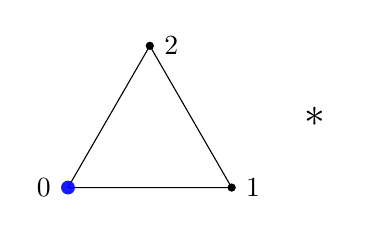
\begin{tikzpicture}[scale=.6]
\coordinate (A) at (210:2);
\coordinate (B) at (-30:2);
\coordinate (C) at (90:2);

\draw[draw=black] (A) -- (B) -- (C) -- (A);

\node[circle,fill=blue, opacity=.9, inner sep=0pt,minimum size=5pt, label=left:{0}] (a) at (A) {};
\node[circle,fill=black,inner sep=0pt,minimum size=3pt, label=right:{$1$}] (a) at (B) {};
\node[circle,fill=black,inner sep=0pt,minimum size=3pt, label=right:{$2$}] (a) at (C) {};

\node[scale=1.5] at (3.5,0.5) {$\ast$};
\end{tikzpicture}
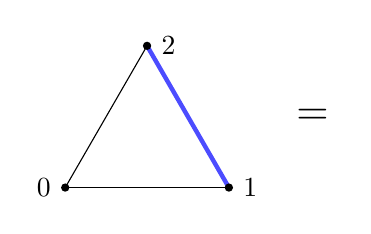
\begin{tikzpicture}[scale=.6]
\coordinate (A) at (210:2);
\coordinate (B) at (-30:2);
\coordinate (C) at (90:2);

\draw[draw=blue, ultra thick, draw opacity=.7] (B) -- (C);
\draw[draw=black] (C) -- (A);
\draw[draw=black] (A) -- (B);

\node[circle,fill=black,inner sep=0pt,minimum size=3pt, label=left:{$0$}] (a) at (A) {};
\node[circle,fill=black,inner sep=0pt,minimum size=3pt, label=right:{$1$}] (a) at (B) {};
\node[circle,fill=black,inner sep=0pt,minimum size=3pt, label=right:{$2$}] (a) at (C) {};

\node[scale=1.5] at (3.5,.5) {=};
\end{tikzpicture}
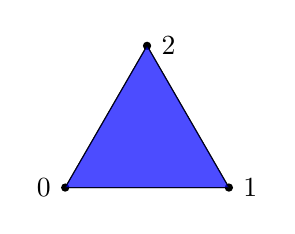
\begin{tikzpicture}[scale=.6]
\coordinate (A) at (210:2);
\coordinate (B) at (-30:2);
\coordinate (C) at (90:2);

\draw[draw=black] (A) -- (B) -- (C) -- (A);

\node[circle,fill=black,inner sep=0pt,minimum size=3pt, label=left:{$0$}] (a) at (A) {};
\node[circle,fill=black,inner sep=0pt,minimum size=3pt, label=right:{$1$}] (a) at (B) {};
\node[circle,fill=black,inner sep=0pt,minimum size=3pt, label=right:{$2$}] (a) at (C) {};

\draw[draw, fill=blue, opacity=.7] (A) -- (B) -- (C) -- (A);
\end{tikzpicture}
	\caption{Geometric representation of the join product of two basis elements. It depicts the identity $\pr \big( [0] \otimes [1,2] \big) = [0,1,2]$.}
	\label{f:join of faces}
\end{figure}
	% !TEX root = ../msimplicial.tex

\section{Comparison with the simplicial theory}\label{s:comparison}

We will use $\sSet$ to denote the category of $1$-fold multisimplicial sets $\mSet{1}$ referring to its objects and morphisms as simplicial sets and simplicial morphisms as usual.

\subsection{Diagonal simplicial set}\label{ss:diagonal}

For any $k \in \N$, the diagonal
\[
\simplex^\op \xra{\diag}
(\simplex^\op)^{\times k} \xra{\cong}
(\simplex^{\times k})^{\op}
\]
induces a functor
\[
(-)^{\diag} \colon \mSet{k} \to \sSet
\]
explicitly defined on a $k$-fold multisimplicial set $X$ by
\begin{gather*}
	X^{\diag}_m = X_{m, \dots, m},
	\qquad
	\face_i = \face_i^1 \circ \dots \circ \face_i^k,
	\qquad
	\dege_i = \dege_i^1 \circ \dots \circ \dege_i^k.
\end{gather*}
It is straightforward to verify that
\[
\big(\simplex^{n_1,\dots,n_k}\big)^\diag \cong
\msimplex{n_1}{n_k}
\]
as simplicial sets.

The functor $(-)^\diag \colon \mSet{k} \to \sSet$ admits a right adjoint $\radj \colon \sSet \to \mSet{k}$, defined, as usual, by the expression
\[
\radj(Y)_{m_1,\dots,m_k} =
\sSet\big( \simplex^{m_1} \times \dots \times \simplex^{m_k}, \, Y \big).
\]
These functors define a Quillen equivalence.
A proof of this fact can be given using \cite[Proposition~1.6.8]{maltsiniotis2005grothendieck}.

\subsection{Eilenberg--Zilber map}\label{ss:eilenber-zilber}

Recall that an \textit{$(n_1,\dots,n_k)$-shuffle} $\sigma$ is a permutation in $\sym_n$ satisfying
\begin{gather*}
	\sigma(1) < \dots < \sigma(n_1), \\
	\sigma(n_1+1) < \dots < \sigma(n_1+n_2), \\
	\vdots \\
	\sigma(n-n_k-1) < \dots < \sigma(n),
\end{gather*}
where $n = n_1+\dots+n_k$.
We denote the set of such permutations by $\sh_{n_1,\dots,n_k}$.
For any $\sigma \in \sh_{n_1,\dots,n_k}$ the inclusion
\[
\gi_\sigma \colon \gsimplex^n \to \gmsimplex{n_1}{n_k}
\]
is defined by the assignment
\[
(x_1,\dots,x_n) \mapsto (x_{\sigma^{-1}(1)}, \dots, x_{\sigma^{-1}(n)}).
\]
If $e$ is the identity permutation, we denote $\gi_{e}$ simply as $\mathfrak{i}$.
The set $\set{\gi_\sigma \mid \sigma \in \sh_{n_1,\dots,n_k}}$ defines a triangulation of $\gmsimplex{n_1}{n_k}$ making it isomorphic, in the category cellular spaces, to the geometric realization of the simplicial set $\msimplex{n_1}{n_k}$.
Using this identification, the identity map induces a cellular map
\[
\ez \colon \gmsimplex{n_1}{n_k} \to \bars[\big]{\msimplex{n_1}{n_k}},
\]
whose induced chain map
\[
\EZ \colon \chains(\simplex^{n_1,\dots,n_k}) \to \chains\big(\msimplex{n_1}{n_k}\big),
\]
agrees, under the natural identifications, with the traditional Eilenberg--Zilber map.

For a multisimplicial set $X$, the induced chain map $\EZ \colon \chains(X) \to \chains(X^\diag)$ is explicitly given on an $(n_1,\dots,n_k)$-multisimplex $x$ by
\[
\EZ(x) \ = \sum_{\qquad \crampedclap{\sigma \in \sh_{n_1,\dots,n_k}}} \sign(\sigma) \, X(\sigma_1 ,\dots, \sigma_k)(x)
\]
%\[
%\EZ \big( [n_1] \times\dots\times [n_k] \big) =
%\sum_{\sigma \in \sh_{n_1,\dots,n_k}} \sign(\sigma) \, \sigma_1 \times\dots\times \sigma_k
%\]
where, for $\ell \in \set{1,\dots,k}$, the morphisms $\sigma_\ell \colon [n] \to [n_\ell]$ are defined by the following property: For
each $j \in \set{1,\dots,n}$ there is exactly one $\ell \in \set{1,\dots,k}$ such that $\sigma_\ell(j+1) = \sigma_\ell(j)+1$ and $\sigma_i(j+1) = \sigma_i(j)$ for all $i \neq \ell$.
\todo{@andrea: this is off, unfortunately. Could you please fix it?}

Since the traditional Eilenberg--Zilber map preserves counital coalgebra structures we have the following.

\begin{theorem*}
	For every multisimplicial set $X$ the map $\EZ \colon \chains(X) \to \chains(X^\diag)$ is a quasi-isomorphism of counital coalgebras.
\end{theorem*}

%\begin{proof}
%	Consider an $(n_1,\dots,n_k)$-multisimplex $x$ with characteristic map
%	\[
%	\zeta \colon \msimplex{n_1}{n_k} \to X.
%	\]
%	The statement follows from the fact that $\EZ(x) = \chains \zeta^\diag \circ \EZ \big([n_1] \ot\dots\ot [n_k]\big)$ and that the usual Eilenberg--Zilber map is a counital coalgebra morphisms.
%\end{proof}

We remark that the Eilenberg--Zilber map is not a morphisms of $E_\infty$-coalgebras.
For example, as shown in \cite[\S5.4]{medina2022cube_einfty}, we have
\[
\Delta_1 \circ \EZ\big([0,1] \ot [0,1]\big) \neq
\EZ \, \circ \, \Delta_1\big([0,1] \ot [0,1]\big).
\]

\subsection{Canonical inclusion}\label{ss:inclusion}

Let $Y$ be a simplicial set and $n$ an integer.
Consider the function $Y_n \to \cU Y_{n,0,\dots,0}$ sending a simplex with characteristic map $\zeta \colon \simplex^n \to Y$ to the composition
\[
\simplex^n \times \msimplex{0}{0} \xra{\pi_1} \simplex^n \xra{\zeta_y} Y.
\]
These functions induce a chain map
\[
\In \colon \chains(Y) \to \chains(\cU Y)
\]
and we have the following.

\begin{theorem*}
	The canonical inclusion $\In \colon \chains(Y) \to \chains(\cU Y)$ is a quasi-isomorphism of $E_\infty$-coalgebras for any simplicial set $Y$.
\end{theorem*}

\begin{proof}
	The structure preserving properties of this map are immediate.
	It remains to be shown that it induces a homology isomorphism.
	Consider the composition of quasi-isomorphisms
	\[
	\chains(\cU Y) \xra{\EZ}
	\chains\big((\cU Y)^\diag\big) \to
	\chains(Y)
	\]
	where the second map is induced by the counit of the adjunction.
	We will now verify that it is left inverse to $\In$.
	Consider a simplex $y$ with characteristic map $\zeta \colon \simplex^n \to Y$.
	The multisimplex $\In(y)$ is given by the simplicial map $\simplex^n \times \msimplex{0}{0} \xra{\pi_1} \simplex^n \xra{\zeta} Y$.
	Since the only $(n,0,\dots,0)$-shuffle is the identity, the simplex $\EZ \circ \In (y)$ is the simplicial map
	\[
	\zeta \circ \pi_1 \colon \simplex^n \times \msimplex{n}{n} \to Y.
	\]
	Finally, the image of this simplex under the counit is the evaluation of $[n] \times\dots\times [n]$ on $\zeta \circ \pi_1$ which gives $\zeta[n] = y$ as claimed.
\end{proof}

\subsection{Singular chains}\label{ss:singular}

\begin{theorem*}
	Let $\fZ$ be a topological space.
	The chain map
	\[
	\rS(\fZ) \to \rS^{(k)}(\fZ),
	\]
	defined by precomposing a continuous map $(\gsimplex^n \to \fZ)$ with the projection
	\[
	\gsimplex^n \times \gmsimplex{0}{0} \xra{\pi_1} \gsimplex^n,
	\]
	is a quasi-isomorphism of $E_\infty$-coalgebras.
\end{theorem*}

\begin{proof}
	This map factors as the composition of two quasi-isomorphism of $E_\infty$-coalgebras.
	The first is $\In \colon \rS(\fZ) \to \chains(\cU^{(k)} \Sing(\fZ))$, which was studied in \cref{ss:inclusion}.
	The second is induced from a multisimplicial isomorphism
	\[
	\cU^{(k)} \Sing(\fZ) \to \Sing^{(k)}(\fZ)
	\]
	defined as follows.
	Using the adjunction of \cref{ss:geometric realization}, any simplicial map $\msimplex{n_1}{n_k} \to \Sing(\fZ)$ corresponds canonically to a continuous map $\bars{\msimplex{n_1}{n_k}} \to \fZ$, which precomposing with $\ez$ gives a continuous map $\gmsimplex{n_1}{n_k} \to \fZ$.
	It is not hard to see that every such map arises this way since $\ez$ is a homeomorphism.
\end{proof}
	% !TEX root = ../msimp.tex

\section{\pdfEinfty-models of configuration spaces}

We are interested in modeling algebraically the equivariant homotopy type of the configuration space of $r$ labeled points in Euclidean $d$-dimensional space.
Multisimplicial sets can be used to provide an explicit chain complex model with a small number of generators.
By Mandell's theorem \cite{mandell2006homotopy_type} and the $E_\infty$-structure introduced in \cref{ss:e-infty extension} this model retains all homotopical information.

\subsection{Recognition of configuration spaces}\label{ss:recognition}

Let $\conf{r}{d}$ denote the configuration space of $r$-tuples of pairwise disjoint vectors in $\R^{d}$.
This space is equipped with a free action of the symmetric group $\sym_r$ of permutations of $\{1,\dots,r\}$ swapping elements of a $r$-tuple.

\begin{definition}
	A \textit{complete graph} on $r$ vertices is a pair $(\mu,\sigma)$ with $\mu$ a collection of non-negative integers $\mu_{ij}$ for all $1 \leq i < j \leq r$, and $\sigma$ is an ordering of $\{1,\dots,r\}$.
	We write $\sigma_{ij}$ for the restriction of the ordering $\sigma$ to the set $\{i,j\}$.
	Graphically $(\mu,\sigma)$ is a simple directed graph in the edge corresponding to $i<j$ directed according to $\sigma_{ij}$ and labeled by $\mu_{ij}$.
	Please consult \cref{f:complete graph} for a example.
	Let us denote the set of complete graphs with $r$ vertices by $\CG(r)$ equipped with the poset structure
	\begin{equation*}
		(\mu,\sigma)\le (\nu,\tau) \ \ \text{ if and only if } \ \
		(\mu_{ij}<\nu_{ij}) \ \ \text{ or } \ \
		(\mu_{ij},\sigma_{ij})= (\nu_{ij},\tau_{ij})
	\end{equation*}
	for each pair $i<j$.
	It is equipped with a filtration by subposets
	\[
	\CG_1(r) \subset \CG_2(r) \subset \dotsb
	\]
	where $\CG_n(r)$ consists of those graphs with $\max(\mu_{ij})< n$.
\end{definition}

\begin{figure}
	\centering
	\begin{equation*}
		\begin{tikzcd}
			\ & 2 & \ \\
			1 \arrow[ur,"2"] \arrow[rr] \arrow[dr,"3"']& \arrow[r,"1"] \arrow[u,"2"] & 3 \arrow[ul,"1"'] \\
			\ & 4 \arrow[ur,"4"'] \arrow[uu] & \
		\end{tikzcd}
	\end{equation*}
	\caption{A complete graph on 4 vertices with ordering $\sigma=(1432)$ and $\mu=(\mu_{12},\mu_{13},\mu_{14},\mu_{23},\mu_{24},\mu_{34})=(2,1,3,1,2,4)$.}
	\label{f:complete graph}
\end{figure}

\begin{definition}
	For a given poset $A$, a cellular $A$-decomposition of a topological space $X$ is a family of subspaces $X_a \subseteq X$ indexed by $a \in A$ such that:
	\begin{itemize}
		\item $a \leq b$ implies $X_a \subseteq X_b$;
		\item $\bigcup_{a \in A} X_a = X$;
		\item $X_a$ is contractible for each $a$;
		\item $\bigcup_{a<b} X_a \subset X_b$ is a closed cofibration.
	\end{itemize}
\end{definition}

\begin{proposition}
	If a topological space $X$ admits a \textit{cellular $A$-decomposition}, then there is a homotopy equivalence between $X$ and the geometric realization of $A$.
	\todo{@andrea,@paolo: We need a reference for this proposition. Is this Quillen's theorem A? I am also happy with saying something like: well know result of McCord ’66 and Quillen ’73 ... Also, I think this statement should be of the form: then the natural map ??? is a homotopy equivalence.}
\end{proposition}

The case of interest for us is the following.

\begin{proposition}[{\cite[\S1.13]{berger1997confspacemodel}}]\label{p:berger}
	If a space has a cellular $\CG_d(r)$-decomposition then it is homotopy equivalent to
	the configuration space
	$\conf{r}{d}$.
\end{proposition}

We warn the reader that configuration spaces themselves do not admit a cellular decomposition with respect to graph complete posets, but they do so with respect to some extended versions of these posets \cite{beuckelmann2021master}.
\begin{equation}\label{eq:extended complete graph map}
	...
\end{equation}
\todo{@andrea,@paolo: We therefore have natural homotopy equivalences ??? for each r and d.}
\subsection{Multisimplicial model} \label{ss:multisimplicial model}

We define for each positive integer $k$ a family of multisimplicial sets $\sur(k)$ equipped with a complete graph filtration
\[
\sur(k,0) \subset \sur(k,1) \subset \sur(k,2) \subset \dotsb
\]
which, by applying to it the functor of chains, recovers the algebraic models of configuration spaces developed by McClure--Smith \cite{mcclure2003multivariable}.

Also the geometric realizations $\mathcal{F}(k) = \bars{\sur(k)}$ appear in the work by McClure-Smith \cite{MS}, as explained in the appendix of \cite{Deligne}.
\todo{@paolo: this sentence appears cryptic to me. Can you say what you mean? Maybe in the previous sentence we can say not algebraic models but ``space'' level.}

Let $\sur(k)$ be the $k$-fold multisimplicial set that has as $(m_1,\dots,m_k)$-multisimplices
the surjective maps
\[
f \colon \set{1,\dots,m+k} \to \set{1,\dots,k}
\]
where $m = m_1+\dots+m_k$ satisfying that the cardinality of $f^{-1}(\ell)$ is $m_\ell$ for each $\ell \in \set{1,\dots,k}$.
We represent this multisimplex by the sequence $f(1) \dotsm f(m+k)$.
The face and degeneracy maps $d^\ell_j$ and $s^\ell_j$ act on it by respectively removing and doubling the $(j+1)^\th$ occurrence of $\ell$ in the sequence.
For example,
\begin{align*}
	d^2_0(12321)&=1321, & s^1_0(121)&=1121, \\
	d^2_1(12321)&=1231, & s^1_1(121)&=1211.
\end{align*}
Degenerate multisimplices are exactly the sequences containing two equal adjacent terms.
A surjection belongs to $\sur(k,d)$ if any ordered subsequence with two distinct alternating values has length at most $d+1$.
For example, $x = 12132 \in \sur_3(3)$ but $x \notin \sur_2(3)$ because the subsequence $1212$ has length 4.
This is a complete graph filtration since...
\todo{@paolo: verify the conditions of complete graph filtration to get the (now commented out) proposition below}
The symmetric group $\Sigma_k$ acts on $\sur(k)$ by post-composition and the action preserves the filtration.

%\begin{proposition} \label{sur-real}
%	There is a $\Sigma_k$-equivariant homotopy equivalence
%	$\bars{\sur_d(k)} \simeq F_k(\R^d)$
%\end{proposition}
%
%\begin{proof}
%	The geometric realization $\bars{\sur_d(k)}$ appears in section 13 of \cite{MS} where it is denoted $Z_0^k$.
%	McClure and Smith define for each $d$ a topological operads $\mathcal{D}_d$ such that $\mathcal{D}_d(k)$ is $\Sigma_k$-homeomorphic to $\bars{\sur_d(k)} \times Tot(\Delta^*)$, where $Tot(\Delta^*)$ is contractible and equipped with trivial $\Sigma_k$-action.
%	This is explained in the appendix of \cite{cyclic} where the realization is constructed as a CW complex and denoted $\mathcal{F}_d(k)$.
%	McClure and Smith proceed to constructing a zig-zag of weak equivalences of operads between $\mathcal{D}_d$ and the little $d$-cubes operad
%	$\mathcal{C}_d$, that in particular gives a levelwise $\Sigma_k$-equivariant equivalence $\mathcal{D}_d(k) \simeq \mathcal{C}_d(k)$ for each $k$. It is well known that $\mathcal{C}_d(k)$ is $\Sigma_k$-equivariantly homotopy equivalent to $F_k(\R^d)$ and this concludes the proof.
%\end{proof}


%The functor of chains applied to these multisimplicial sets induces chain complex $\chi(k,d) \defeq \chains(\sur(k,d))$ with a filtration
%\[
%\chi(k,0) \subset \chi(k,0) \subset \chi(k,2) \subset \dotsb,
%\]
%which were considered by McClure and Smith \cite{MS}, %actually other paper
%who constructed an operad structure on the collections of these complexes, the {\it surjection operad} $\chi$.
%gives a filtration of the surjection operad by suboperads
%$$\chi_0 \subset \chi_1 \subset \chi_2 \subset \dots \subset \chi$$

\begin{theorem*}
	For any configuration space $\con(r,d)$ the maps in the following zig-zag are $\sym_r$-equivariant quasi-isomorphisms of $E_\infty$-coalgebras, or more precisely of $\UM$-coalgebras:
	\[
	\schains\con(r,d) \leftarrow \schains \cgr(r,d) \to \schains\bars{\sur(r,d)} \to \schains^{(r)}\bars{\sur(r,d)} \leftarrow \chains(\sur(r,d))
	\]

\end{theorem*}

\begin{proposition} \label{sur-model}
	$\chi_d(k)$ and $\rS{F_k(\R^d)}$ are $\Sigma_k$-equivariantly quasi-isomorphic $E_\infty$-coalgebras
\end{proposition}

\begin{proof}
	The $\Sigma_k$-equivariant homotopy equivalence of proposition \ref{sur-real} induces a $\Sigma_k$-equivariant quasi-isomorphism of $E_{\infty}$-coalgebras
	$$S^{(k)}(\bars{\sur_d(k)}) \simeq S^{(k)}(F_k(\R^d))$$.
	The weak equivalence %say that it is Quillen adjunction
	$\sur_d(k) \to Sing^{(k)}(\bars{\sur_d(k)})$ induces on the chain level a $\Sigma_k$-equivariant quasi-isomorphism of
	$E_\infty$-coalgebras
	between $\chi_d(k)$
	and $S^{(k)}(\bars{\sur_d(k)})$.
	Finally the map of lemma \ref{} gives a $\Sigma_k$-equivariant quasi-isomorphism $S^{(1)}(F_k(\R^d)) \to S^{(k)}(F_k(\R^d))$ of $E_\infty$-coalgebras.
\end{proof}

% !TEX root = ../msimp.tex

\subsection{Simplicial model}\label{ss:simplicial model}

We recall the Barratt--Eccles simplicial set $\BE(r)$ defined for each $r\in\N$ that is equipped with a $\CG(r)$-filtration.
Applying the functor of chains to the nested sequence
\[
\BE_{1}(r) \subset \BE_{2}(r) \subset \dotsb.
\]
will provide the algebraic models
\[
\cE_{1}(r) \subset \cE_{2}(r) \subset \dotsb
\]
of configuration spaces studied by Berger and Fresse in \cite{berger2004combinatorial}.

The $n$-simplices of $\BE(r)$ are tuples of $n+1$ elements of the symmetric group $\sym_r$.
Its face and degeneracy maps are defined by removing and doubling elements respectively.
There is an operad structure on these simplicial sets, but we do not consider it here.

Next we recall a $\CG(r)$-filtration on $\BE(r)$.
For $i<j$ and $\sigma$ in $\sym_r$ let $\sigma_{ij}$ be the associated permutation in $\sym_2$.
Given $(\mu,\sigma) \in \CG(r)$ then an
element $w = (w_0,\dots w_n) \in \BE(r)_n$,
$w \in \BE(r)_{(\mu,\sigma)}$ if for each $i<j$, the cardinality of $\set{\ell \mid (w_{\ell})_{ij} \neq (w_{\ell+1})_{ij}}$ is either less than $\mu_{ij}$ or equal to it and $(w_0)_{ij} = \sigma_{ij}$.

In particular $w$ has complexity $d$ or less if for each $i<j$
%the cardinality of $\set{\ell=1,\dots,n-1 \mid w_{\ell-1,ij} \neq w_{\ell,ij}}$ is less than $d$, i.e., 
the non-degenerate dimension of $w_{ij}=((w_0)_{ij},\dots,(w_n)_{ij})$ in $\BE(2)$ is $d$ or less for all $i<j$.
We notice that the action of $\sym_r$ on $\BE(r)$ preserves the nested sequence
$$\BE_1(r) \subset \BE_2(r) \subset \dots$$
For a proof that this is a $\CG(r)$-filtration we refer to Example 2.8 in \cite{berger1997confspacemodel}.
Please consult \cite{smith1989filtration,kashiwabara1993confcomplex,berger1997confspacemodel} for more details.
 
Applying the functor of singular chains to the zig-zag of \cref{p:zig-zag conf} produces a zig-zag of equivariant quasi-isomorphisms of $\UM$-coalgebras connecting $\schains\bars{\BE_d(r)}$ and $\schains\conf{r}{d}$.
Using the unit of the Quillen equivalence extends this zig-zag to one relating $\chains\BE_d(r)$ and $\schains\conf{r}{d}$, which can be combined with the zig-zag constructed in the previous subsection.
As announced in the introduction, this construction relates the chains on the multisimplicial model of configuration space and those the simplicial model via an explicit zig-zag of equivariant quasi-isomorphisms of $E_\infty$-coalgebras.



\subsection{Counting generators}

We stress that the number of generators in $\chi_d(k)$, corresponding to non-degenerate surjections, is much smaller than the corresponding number of generators in $BE_d(k)$.
We give some examples.
Let us consider the generating polynomial functions counting the generators
$$PB_d^k(x) = \sum_i rank(BE_d(k)_i) x^i $$ $$P\chi_d^k(x)=
\sum_i rank(\chi_d(k)_i) x^i$$
Then for example
\begin{align*}
	& PB_2^4(x)=24(1+23x+104x^2+196x^3+184x^4+86x^5+16x^6)\\
	& P\chi_2^4(x)=24(1+6x+10x^2+5x^3) \\
	& \\
	& PB_3^3(x) = 6(1+5x+25x^2+60x^3+70x^4+38x^5+8x^6 ) \\
	&  P\chi_3^3(x)= 6(1+3x+7x^2+9x^3+6x^4+x^5)
\end{align*}
Therefore the multisimplicial approach using $\chi$ is much more efficient than the simplicial
approach using $BE$, when performing computations as in \cite{formality}.


	\sloppy
	\printbibliography
\end{document}